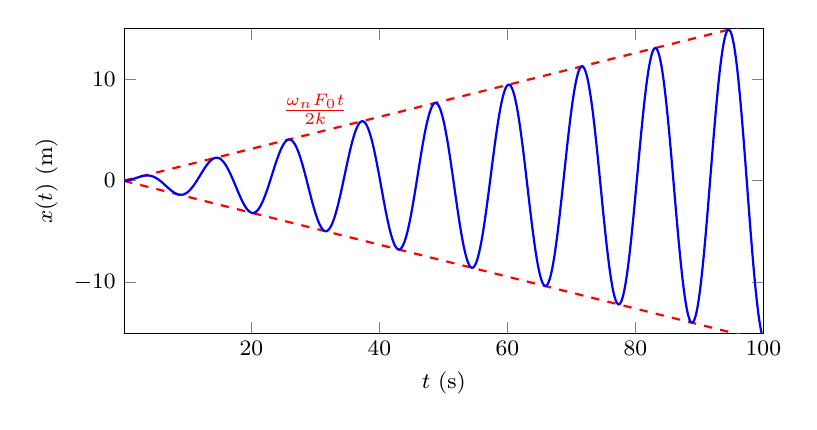
\begin{tikzpicture}[scale=1]
	\footnotesize
	\begin{axis}[
		width=0.8\textwidth,
		height=0.45\textwidth,
		xlabel={$t$ (s)},
		ylabel = {$x(t)$ (m)},
		xmax=100,
		xmin=0.1,
		ymax=15,
		ymin=-15,
		samples=1000]
		
		
		\def\wn{5*2*pi};
		\def\Fo{0.01};
		\def\k{1};
		
		\addplot[red, dashed, thick, domain=0.1:100] (x, {\wn*\Fo*x/(2*\k)});		
		\addplot[red, dashed, thick, domain=0.1:100] (x, {-\wn*\Fo*x/(2*\k)});				
		\addplot[blue, thick, domain=0.1:100] (x, {\wn*\Fo*x/(2*\k)*sin(\wn * x)});

		\node at (axis cs: 30,7) [red] {$\frac{\omega_n F_0 t}{2k}$};
		
		
	\end{axis}
	
\end{tikzpicture}